% !TEX root = ../main.tex
\label{section:results}
\section{Results}

In this section, we compare the performance of the previously introduced models and methods and illustrate the results. They provide insight on the effects of incorporating knowledge about physical constraints and some limitations.

\subsection{Model architecture}
As described in the section \ref{ssec:network_architectures}, we first compare the three introduced network architectures. The performance of the models is displayed in Figure \ref{fig:models}.
\begin{figure}[ht]
	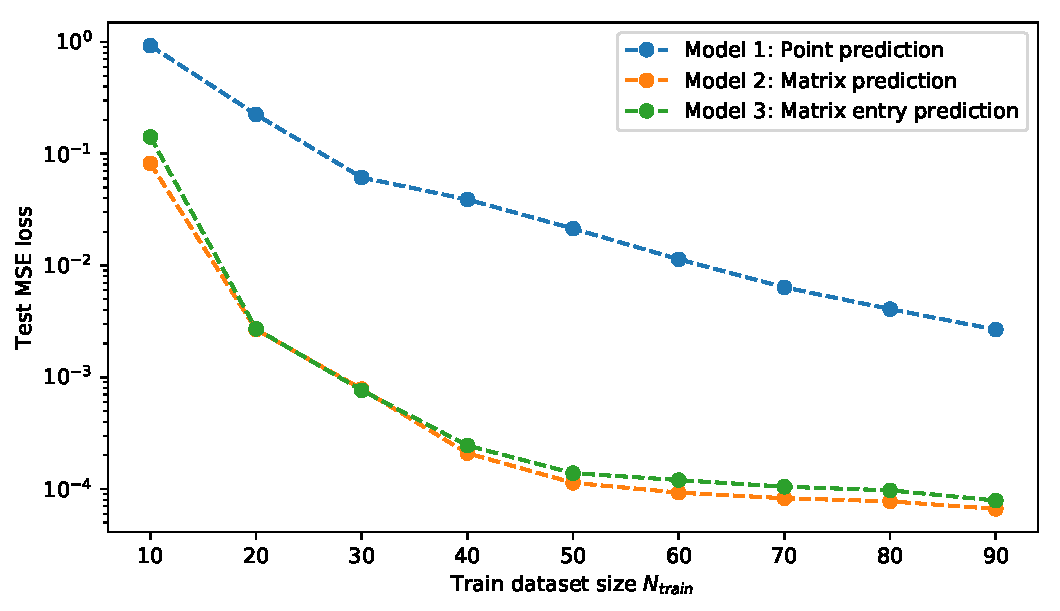
\includegraphics[width=\linewidth]{models}
	\caption{Different model architectures}
	\label{fig:models}
\end{figure}
We can see that while the difference between the behaviours of Model 2 and 3 are quite small, they both perform significantly better than Model 1. This aligns with our expectations, since the latter two models already make use of the knowledge that a rotation can be represented as the multiplication of the point with a matrix that only depends on the rotation angle. Even though both matrix models perform well and almost the same for up to 50 data points, the Model 2 finds a slightly better solution for higher amounts of training data (CHECK IF STILL TRUE FOR 20 RUNS). In order to be able to extract the true effects of the methods we apply, all of the following experiments use one of the well performing models, which we choose to be Model 2. Since it already reaches a Test MSE Loss of almost $10^{-3}$ with 20 training data points and starts to converge only after using more than 6 points, the majority of the following analysis focuses on the interesting region of 10 to 20 as the size of the training dataset. In order to make sure that the improvements of the following methods utilizing the physical constraints are not due to the regularization they entail, we checked that L2-Regularization has no significant or consistent positive impact. The results can be looked up in the appendix in Figure \ref{fig:reg_weights}.

\subsection{Penalty method}
\subsubsection{Fixed physical loss weight}
First, we apply the Penalty Method using a fixed weight $\lambda$ for the detminant physical loss $\mathcal{L}_{DET}$ and therefore only solve a single minimization problem during the training process. The results obtained by this method performing 50000 epochs on the 2D-Rotation problem are shown in Figure \ref{fig:pnlty_det}.

\begin{figure}[ht]
	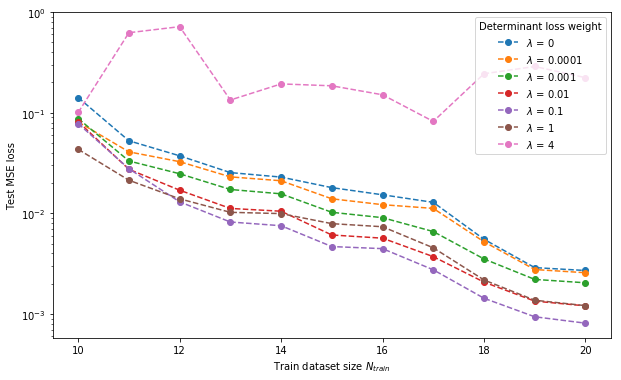
\includegraphics[width=\linewidth]{pnlty_det}
	\caption{Different weights $\lambda$ for $\mathcal{L}_{DET}$}
	\label{fig:pnlty_det}
\end{figure}


Looking at these results, we immediatly observe the method's robustness for different weights of the physical loss, since small weights in a range of at least two orders of magnitude, namely $\lambda \in [0.01, 1]$, lead to significantly improved performance. For smaller values of $\lambda$, the test error converges to the one of $\lambda= 0$, whereas values of $\lambda > 1$ lead to a heavy focus on satisfying the physical constraint and thus leads to poor results compared to smaller values and $\lambda=0$.\\
\indent Moreover, we can see that the choice $\lambda = 0.1$ consistently yields to smaller error on the test dataset. It is also important to note that the performance improvement is significant. For example, with only 20 training data points, the physically trained model achieves a Test MSE Loss of xxx, whereas the model trained solely on the train MSE Loss achieves only a value of yyy, thus reducinf the error by a factor of x. \\
\indent Interestingly, utilizing the penalty method leads to higher performance even for larger train datasets. This can be seen in Figure \ref{fig:pnlty_det_large} in the appendix, displaying the results of an experiment we did for a wider range including up to 100 training data points.\\
We observe similar qualitative behaviour when applying the method for the 3D-rotation, as displayed in Figure \ref{fig:pnlty_det_dim3} in the appendix.\\
\indent However, we are not only interested in the overall test performance, but also how realistic the predictions are. Figure \ref{fig:pnlty_det_analysis} shows the absolute difference of the determinant of the predicted rotation matrix and 1, the absolute difference of the norm of the predicted points and 1, and the test loss, all averaged across numerous points for each angle.\\
\indent First of all, we can see that the desired physical constraint is met perfectly at each training point, which already contributes to smaller overall errors in these regions. Even more important is the effect of the penalty method on predictions in areas where training data is sparse. An interesting region to analize is the one for angles between $0.2$ and $2.2$, where not a single training data point exists. We can observe both smaller deviation of the determinant from one and smaller test error, meaning that the predictions are not only more realistic, but also closer to the true values.
\begin{figure}[ht]
	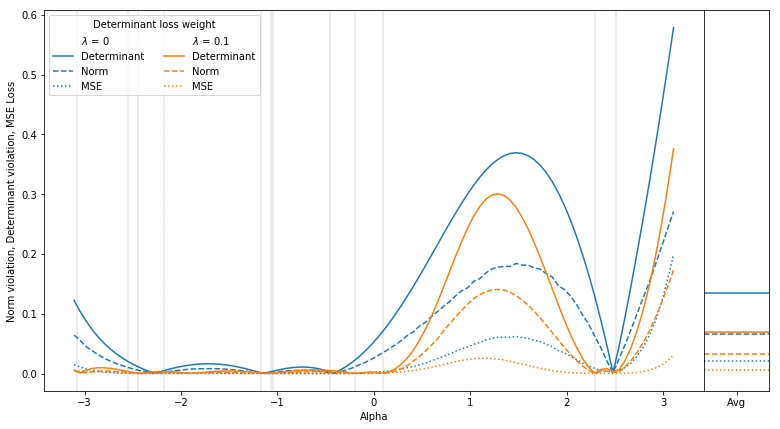
\includegraphics[width=\linewidth]{pnlty_det_analysis}
	\caption{Determinant and norm violations of predictions for $N_{train} = 12$. Gray vertical lines represent the angles of the training points.}
	\label{fig:pnlty_det_analysis}
\end{figure}

\subsubsection{Increasing physical loss weight}
When analyzing the version of the penalty method where we solve a series of minimization problems with increasing weights $\lambda$ for $\mathcal{L}_{DET}$, we first have to discuss finding a good set of parameters. The parameters we need to determine for this method are the following:
\begin{itemize}
	\item Initial weight $\lambda_0 > 0$
	\item Increasement factor $\mu > 1$, determines $\lambda_k = \mu^k\lambda_0$
	\item Condition when to stop the current iteration
	\item Number of iterations
\end{itemize}
In general, we can say that it is difficult finding a successful set of parameters, since we only have an intuition about the initial and last value of $\lambda$. We manually tried several different parameter sets, of which many led to much worse performance than the results shown above. However, we were able to increase performance with the following values: We set $\lambda_0 = 10^{-3}$, $\mu = 1.05$, use 50 iterations and stop the k-th iteration once the norm of the gradient is smaller than $0.95^{k} 10^{-3}$. With this, we get a last weight value of $\lambda_{50} \approx 10^{-2}$. The results are illustrated in Figure \ref{fig:pnly_dyn}. However, since solving a series of minimization problems with the chosen parameters involves approximately $150k$ iterations, we also compare the results with using the fixed method for $150k$ iterations for different values taken by $\lambda$ during the dynamic training process.

\begin{figure}[H]
	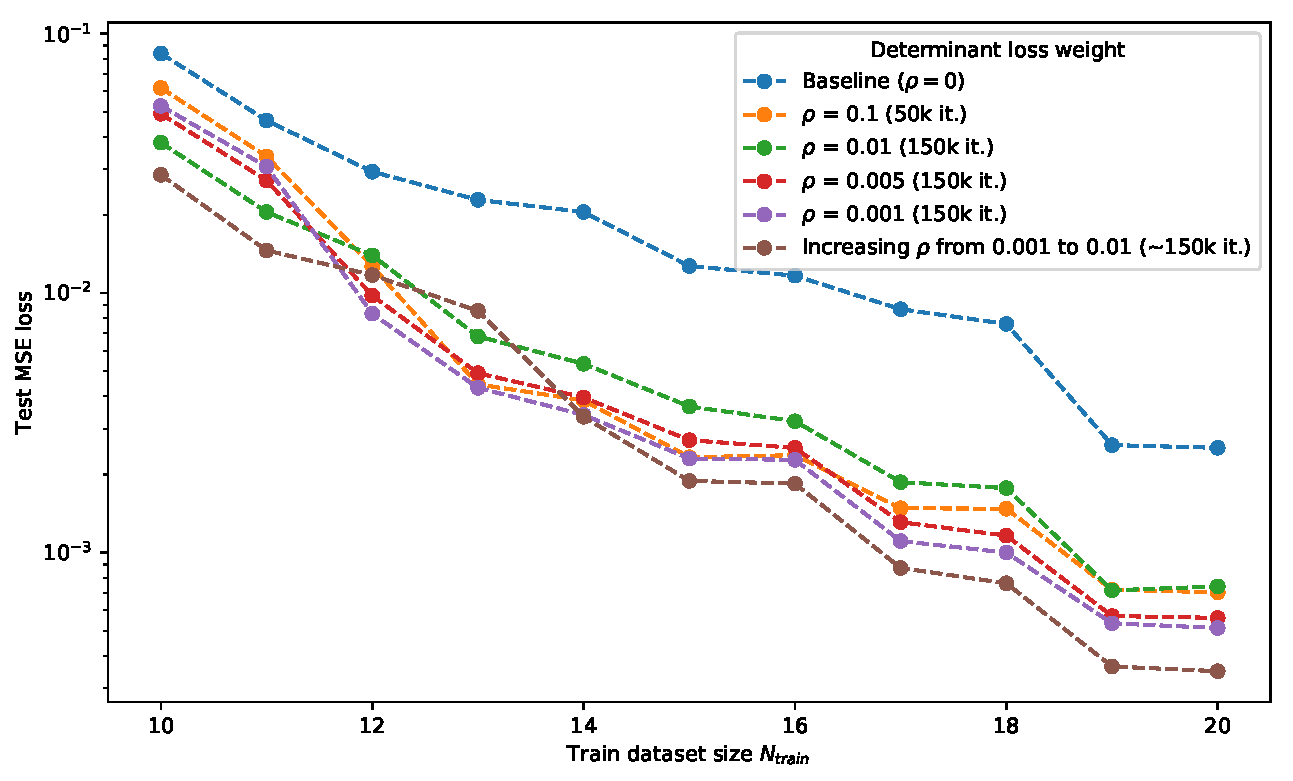
\includegraphics[width=\linewidth]{pnly_dyn}
	\caption{Different weights $\lambda$ for $\mathcal{L}_{DET}$ compared with dynamically increasing $\lambda$}
	\label{fig:pnly_dyn}
\end{figure}

For the chosen parameters, the increasing penalty method achieves higher performance than the fixed one. However, since it requires a multiple of the epochs needed by the fixed method and it is difficult to find a well performing set of parameters, we overall prefer the simpler method using a fixed physical loss weight $\lambda$.

\subsection{Augmented Lagrangian Method}

We first apply the version which only computes a fixed number of epochs for each minimization problem, and keeps the weight $\lambda$ of the physical loss $\mathcal{L}_{DET}$ constant. Thus, it differs from the first version of the Penalty Method only in having the additional linear constraint violation term. Note that for ALM, this weight needs to be chosen significantly smaller than for the Penalty Method depending on the constraint violation, since the linear term is much higher relative to the squared constraint violation term for small violation values. Still, it is similarly difficult to find a good set of parameters as it is for the second version of the Penalty Method. We achieved reasonable performance computing 30 iterations with 5000 epochs each and a physical loss weight of $\lambda = 0.01$. The results are depicted in Figure \ref{fig:aug_lag} as "ALM fixed". In order to clearly extract the effect of incorporating ALM's core idea of including the linear constraint violation terms, we also include "ALM fixed (no linear)", which uses the same loss function, but omitting the linear terms. The results show that by using ALM with a good set of parameters, we can achieve even smaller error rates than the Penalty Method. However, the improvements are not very consistent in the range between 10 and 15 training data points. Further, we have to note that the metod again needs $150k$ epochs in total compared to the $50k$ epochs of the fixed Penalty Method in order to achieve comparable results.
\begin{figure}[H]
	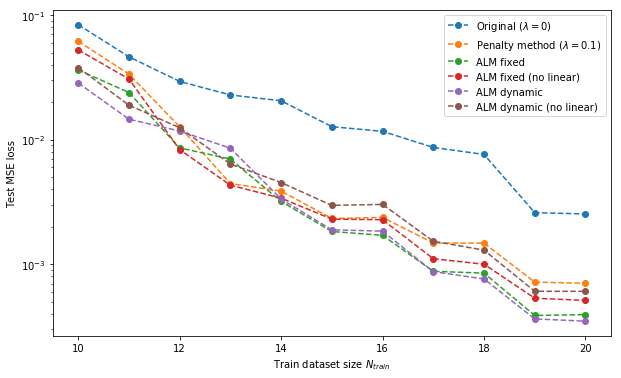
\includegraphics[width=\linewidth]{aug_lag}
	\caption{Comparison of ALM, Penalty Method and original training, averaged over 10 different random training datasets.}
	\label{fig:aug_lag}
\end{figure}
Furthermore, Figure \ref{fig:aug_lag} depicts the results of applying the second version of ALM, again including the comparison with the same computation without the linear term in the loss function. As described in section \ref{exp:alm}, we need to determine even more parameters than we do for the first version of ALM or the Penalty Method. This makes it especially difficult to find good parameters, and we need to mention that throughout the process of finding a good parameter set, we have tried many values that led to significantly worse performance than the original model which does not incorporate any physical constraints at all. To get reasonable results, we chose the following parameters: To begin with, we set $\lambda_{0} = 10^{-3}$ and increased it by a factor of $1.05$ after each iteration. By computing 50 iterations, $\lambda$ increases by approximately one order of magnitude. In order to make use of the proposed idea of setting the gradient threshold to a minimum of a fixed value and one dependent on the constraint violation, we set $\gamma_k = 0.95^k\,10^{-1}$ and $\epsilon_k = 0.95^k\,10^{-3}$. These values were chosen after analyzing the constraint violation values during training and set such that $\epsilon_k$ and $\gamma_k ||c(x_k)||$ have approximately the same order of magnitude. The achieved results using these parameters are similiar to the fixed ALM results, and again achieve smaller error rates than the corresponding training omitting the linear term. However, also this version of ALM does not perform consistently better than the Penalty Method. Furthermore, it needs at least $150k$ and up to $300k$ epochs to achieve these results.\\
\indent To understand the impact of ALM on how well the predictions align with the physical constraints, Figure \ref{fig:alm_det_analysis} depicts the absolute difference of the prediction norms and one, the absolute difference of the determinant of the predicted rotation matrix and one, and the corresponding MSE Loss. Note that results vary and Figure \ref{fig:alm_det_analysis} only depicts the values for 12 training data points and a single seed used to generate the training dataset.

\begin{figure}[H]
	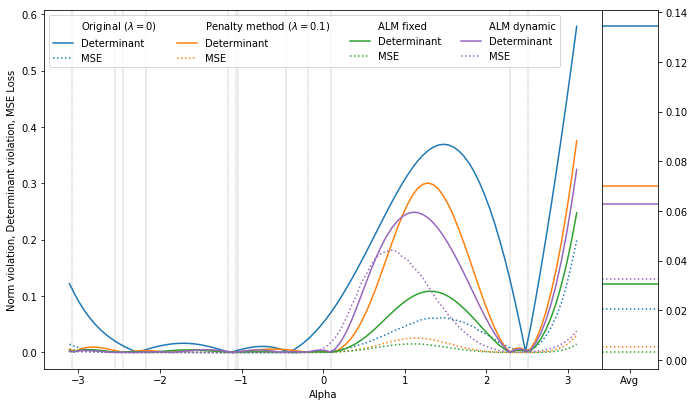
\includegraphics[width=\linewidth]{alm_det_analysis}
	\caption{Determinant and norm violations of predictions for $N_{train} = 12$. Gray vertical lines represent the angles of the training points.}
	\label{fig:alm_det_analysis}
\end{figure}

As expected knowing the statistical performance of the methods, the deviations from the physical constraints are significantly smaller when we apply one of the proposed methods compared to the original training. Similar to the Penalty Method, both versions of the Augmented Lagragian Method lead to no constraint violations at points where training data is present. While the fixed ALM in this case generalizes the physical constraints significantly better than the Penalty Method, the dynamic version achieves only comparable results. Despite, an interesting observation is the high MSE Loss average of the dynamic ALM, which exceeds with a value of 0.033 the error of all other methods significantly. Even the original model achieves an overall average of the MSE Loss of 0.21. However, this is only due to the performance in the range of angles between 0 and 2, for the extrapolation of angles higher than 2.5, it performs much better than the original model. This is the case even though the determinant in the difficult region is much closer to one than the determinant of the prediction of the original model. This indicates that the ALM focused too much on learning the determinant constraint, since it is able to generalize the determinant only at cost of the performance of the predictions.\\
\indent Furthermore, we want to point out that finding a good condition when to stop the training process is difficult. The test performance throughout the training process for different randomly generated training datasets is depcited in Figure \ref{fig:test_training}. When comparing the performance of the Penalty Method (left) with the Dynamic ALM (right), we can instantly see much higher deviations when using the latter method. For example, the test performance colored in blue reaches a test MSE Loss of less than $0.7\times 10^{-4}$, but only achieves an error of more than $3\times 10^{-2}$ when training has ended. In contrast, most of the test errors of using the Penalty Method converge and following epochs only lead to slight overfitting. This in turn indicates the high potential of ALM as well. As we can see, the best performance achieved often exceeds the final performance significantly. More sophisticated methods used to determine the hyperparameters of ALM  might therefore lead to much higher improvements compared to what we achieve with the current parameters.
\begin{figure}
	\centering
	\begin{subfigure}{.5\textwidth}
		\centering
		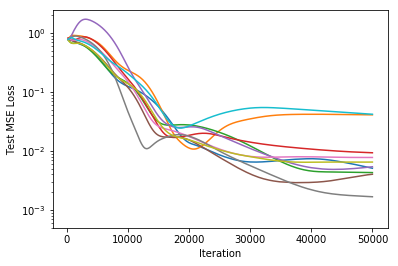
\includegraphics[width=\linewidth]{rand_test_pnlty}
		\caption{Penalty method with $\lambda = 0.1$}
	\end{subfigure}%
	\begin{subfigure}{.5\textwidth}
		\centering
		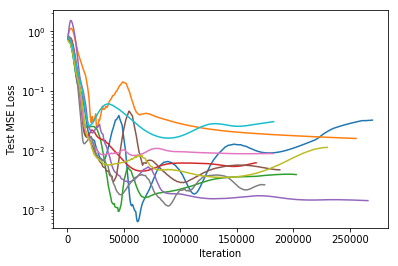
\includegraphics[width=\linewidth]{rand_test_alm_dyn}
		\caption{Dynamic ALM}
	\end{subfigure}
	\caption{Test error throughout the training process, each color represents a different training dataset.}
	\label{fig:test_training}
\end{figure}





\clearpage

